%===========================================
\chapter{Premiers programmes}
%===========================================

La traduction d'un algorithme en un programme est une première étape de
développement. La réalisation — c'est-à-dire l'exécution du programme sur une
machine — est une seconde étape très importante. Que faut-il faire en plus de la
traduction de l'algorithme pour que le programme fonctionne sur un ordinateur ? 

\minitoc

%
%
%
%
\section{Introduction}

Il existe beaucoup de langages de programmation. Ces langages peuvent être
rassemblés par classes de langages en fonction de leurs spécificités. Une classe
de langages est adaptée à une classe de problèmes. Les langages — comme les 
problèmes — évoluent au fur et à mesure du temps. 

\begin{description}
	\item[langage machine]
		le langage machine est le langage de plus bas niveau. Il est exécutable 
		par la machine et incompréhensible par l'humain sans effort;
	
	\item[langage assembleur]
		là où tout est représenté par des nombres en langage machine, le langage
		assembleur propose une première couche d'abstraction~: les instructions
		sont des mots~: \pc{MOV}, \pc{JMP}… 
	
	\item[langage de haut niveau]
		
		les langages de haut niveau sont destinés aux développeurs, le niveau
		d'abtraction est grand. Ils proposent des instructions, des variables,
		des structures de contrôle… tout ça sera traduit pour être compris par
		la machine. 
		
		Par exemple, \textit{Fortran, COBOL,Pascal, C…}
	
	\item[langage orienté objets]

		là où les langages de haut niveau étaient plus orientés sur les problèmes
		à résoudre 
		
		— Que faut-il faire~? 
		
		les langages orienté objets s'intéressent d'abord aux données 
		
		— Quelles sont les données que nous avons et que devons nous fournir~? 
		
		C'est sans doute la classe de langages la plus répandue. 
		
		Par exemple, {\it C++, Java, C\#, Python, Go, Ruby, VB.NET, Vala,}
		\textit{Objective C, Eiffel, Ada, PHP, Smalltalk, Scala… }

	\item[langage fonctionnel]

		là où les langages orienté objets s'intéressent aux changements d'état 
		des objets lorsqu'ils évoluent au fur et à mesure du programme, la 
		programmation fonctionnelle consiste à exprimer le problème à résoudre en 
		terme de fonctions (mathématiques). C'est une autre façon de programmer. 
		Si elle est peu répandue, elle n'est pourtant pas récente.

		Par exemple, \textit{Lisp, Common Lisp, Haskell, Scala…}

\end{description}

Dans ce cours, nous nous intéressons au langage orienté objets, Java.

La langage Java est un langage strict. Il impose, par exemple, que l'on déclare
les variables que l'on utilise et il vérifie que les données assignées aux
variables soient du «~bon~» type. Il possède un \textit{garbage collector}
(ramasse-miettes en français\footnote{Vous noterez la traduction.}) qui gère la
mémoire à la place du développeur. Ces aspects facilitent l'acquisition de bonnes
pratiques de développement. 

C'est également un langage très présent dans l'industrie. Il est donc bien
adapté pour des étudiants entamant un \textit{bachelor} professionnalisant.

Certaines personnes lui reprocheront sa lenteur et sa syntaxe qui peut paraitre 
lourde au premier abord tandis que d'autres rétorqueront que la lenteur n'est due
qu'à la mauvaise qualité du code.

Vous aurez tout le loisir de vous faire votre propre idée. 

%
%
\subsection{Compilation - interprètation}
\label{compilation-interprètation}

L'ordinateur ne comprenant que le langage machine, toutes les instructions
devront, à un moment ou à un autre, être traduite en langage machine. Pour
certains langages, la traduction se fait une fois pour toutes. Ils sont
compilés. Pour d'autres la traduction se fait au \textit{fil de l'eau}, pendant
l'exécution. Ils sont interprétés. 


\clearpage
\index{compilation}
\marginicon{definition}
\textbf{Définition} 

Un langage est \textbf{compilé} (voir fig. \ref{compilé}) si le code source est
traduit d'une traite. Un nouveau fichier contenant le code exécutable est créé. 

Ces langages nécessitent un \textbf{compilateur}. 

\begin{figure}[h]
\begin{center}
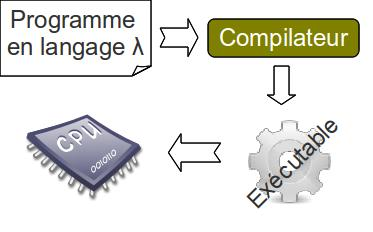
\includegraphics[width=9cm]{images/java-jvm-compil}
\caption{Langage compilé}
\label{compilé}
\end{center}
\end{figure}

%\pagebreak[4]
\index{interprètation}
\marginicon{definition}
\textbf{Définition}

Un langage est \textbf{interprèté} (voir fig. \ref{interprété}) si le code
source est traduit instruction par instruction. Aucun nouveau fichier n'est créé
et les instructions sont traduites à chaque exécution du programme. 

Ces langages nécessitent un \textbf{interprèteur}\footnote{Certaines personnes 
préfèrent parler d'un interprète mais le terme prête à confusion.}.

\begin{figure}[h]
\begin{center}
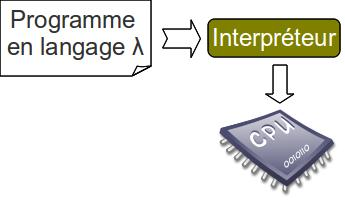
\includegraphics[width=7cm]{images/java-jvm-interp}
\caption{Langage interprété}
\label{interprété}
\end{center}
\end{figure}

Les deux approches ont leurs avantages et leurs inconvénients. 

\begin{itemize}
	
	\item Dès lors qu'une machine possède l'interprèteur, le développeur peut
		diffuser son code et le code pourra être exécuté sur la machine\ldots
		quel que soit son OS (\textit{operating system}, système d'exploitation). 

		Le programme fonctionnera sans modification supplémentaire sur une 
		machine MS Windows, Linux ou Mac OS. 

	\item Avec une approche «~interprétée~», pour diffuser un programme, il faut 
		diffuser le code source. S'il s'agit d'un langage compilé, il est possible
		de ne distribuer que le binaire / exécutable.

		Par contre, il existe des «~\textit{décompilateurs}~» qui peuvent
		reconstruire le code source à partir du binaire / exécutable.

	\item La phase de compilation permet de détecter beaucoup de (petites)
		erreurs avant d'exécuter le programme.

	\item L'exécution du binaire / exécutable est plus rapide que
		l'interprétation du code source. 

\end{itemize}

\marginicon{definition}
Java a une approche mixte, il est compilé et ensuite interprèté. Le code source
est compilé et produit un \textit{bytecode} sauvegardé dans un nouveau fichier.
Le \textit{bytecode} est ensuite interprété par une machine virtuelle, la
\textit{jvm} \index{jvm} (\textit{Java Virtual Machine}). 

\bigskip
\begin{figure}[h]
\begin{center}
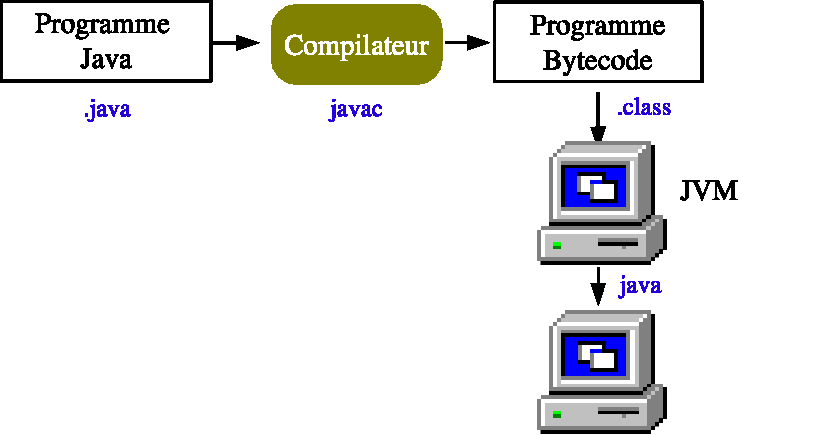
\includegraphics[width=14cm]{images/java-jvm-jvm2}

\caption{Java est compilé et ensuite interprété}
\label{jvm}
\end{center}
\end{figure}

Le \textbf{code source} du programme est écrit dans un fichier texte dont
l'extension sera \texttt{.java}. C'est le fichier que manipule le développeur.
Le code source est la suite d'instructions java. 

À l'aide du \textbf{compilateur} — le programme \texttt{javac} — le fichier est
compilé. Un nouveau fichier ayant comme extension \texttt{.class}, est créé
contenant le \textit{bytecode}.  Ce fichier est destiné à la machine virtuelle.
Voici l'instruction pour compiler le programme.

\begin{term}
	javac MyProgram.java
\end{term}

C'est la machine virtuelle — le programme \texttt{java} — qui est l'interprèteur 
du bytecode. C'est ce programme qui permet d'exécuter le… programme. 

\begin{term}
	java MyProgram
\end{term}

\paragraph{Remarques} 
\label{jdk11}

\begin{enumerate}
	
	\item Notez que \texttt{javac} prend le nom d'un fichier en paramètre (avec
		son extension) alors que \texttt{java} prend le nom d'un programme
		— nous dirons une classe bientôt — en paramètre (sans extension donc). 

	\item Avec JDK11, il est possible de passer un fichier à la commande
		\texttt{java}. Dans ce cas, la commande compilera le fichier, conservera
		le bytecode en RAM et l'exécutera. Il n'y aura donc pas création d'un
		fichier contenant le \textit{bytecode} et le code source sera exécutable
		en une seule commande (voir \cite{pbt-jdk11}).  

		\begin{term}
			java MyProgram.java
		\end{term}

		\textbf{Attention de ne pas confondre.}

\end{enumerate}
 


%
%
%
%
\section{Environnement de développement}

\index{environnement}
L'environnement de développement représente l'ensemble des outils nécessaires au
développement, à l'écriture des programmes. 

\subsection{La base}

Il est évidemment nécessaire d'avoir un \textbf{ordinateur} et de le connaitre 
un tant soit peu. Voici quelques compétences nécessaires~:

\begin{itemize}
	\item manipuler des fichiers~: les déplacer, les trouver, les renommer…
	\item ouvrir un terminal;
	\item connaitre son clavier et particulièrement où se trouvent les caractères
		spéciaux. Par exemple~: \verb|{}[];<>"'|;

\end{itemize}

Par contre, que l'OS utilisé soit MS Windows, linux ou Mac OS importe peu pour 
l'apprentissage de l'algorithmique et du développement en Java. 

\subsection{Écrire le code}

\index{ide}
Pour \textbf{écrire le code}, deux approches sont possibles~: l'utilisation 
d'un éditeur de code ou d'un IDE (EDI, Environnement de Développement Intégré).

\begin{enumerate}
	\item \textbf{éditeur de code}

		Un éditeur de code est un éditeur de texte — à ne pas confondre avec un
		traitement de texte — augmenté c'est-à-dire offrant des fonctionnalités
		supplémentaires. Citons par exemple~:

		\begin{itemize}

			\item la coloration syntaxique. Le programme reconnait les mots clés
				du langage, les structures et les écrit en couleur pour
				accroitre la lisibilité du code;

			\item l'indentation automatique et la réindentation du code;

			\item une certaine autocomplétion pour les mots connus du langage 
				et les variables.

		\end{itemize}

		Exemples d'éditeurs de code toutes plateformes, licences et prix
		confondus~: {\itshape (g)Vim, Notepad++, Atom, SublimeText…}
	
		Exemples d'éditeurs de texte inutiles pour le développement~: {\itshape
		nano, Notepad, Mousepad}.


	\item \textbf{IDE}

		Un environnement de développement intégré est un programme servant à 
		écrire les programmes. En plus d'un éditeur de code, un IDE compile 
		en arrière plan, a un débogueur, organise les fichiers, crée des fichiers
		(en partie) pré-complétés sur base de \textit{templates}…

		Exemples d'IDE~: {\itshape Netbeans, Eclipse, IntelliJ… }

\end{enumerate}

Connaitre et utiliser correctement un éditeur de code et un IDE sont deux
compétences essentielles d'un bon développeur. L'une n'allant pas sans l'autre. 

\subsection{Exécuter le programme}

Quand le code est écrit, il faut le compiler puis l'exécuter. Les deux
programmes, \texttt{javac} et \texttt{java}, font partie d'un ensemble de
programmes fournis avec le langage Java. Cet ensemble de programmes nécessaires
au développement en Java s'appelle \textbf{JDK}~:\textit{Java Development Kit}
\index{JDK}

Il en existe deux~:

\begin{enumerate}
	
	\item Java est — actuellement — la propriété d'Oracle et c'est Oracle qui
		fournit le JDK officiel. 

		\href{http://www.oracle.com/technetwork/java/javase/downloads}
		{Télécharger Java chez Oracle}

	\item OpenJDK est une alternative libre au JDK officiel Java.

		\href{http://openjdk.java.net/}{Télécharger OpenJDK}

\end{enumerate}


\paragraph {Remarque} Il ne faut pas confondre JDK et JRE\index{JRE}. Un JRE
pour \textit{Java Runtime Environment}, est l'ensemble de programmes — il y en
a moins — nécessaires à l'\textbf{exécution} de programmes Java. Dans ces
programmes se trouve une machine virtuelle java (\textit{JVM}) pour
l'interprètation des programmes java. 

Vous avez probablement déjà un — voire plusieurs — JRE sur votre machine. 


\subsection{Hello world}
\label{helloworld}

Une fois les armes fourbies, il est temps d'écrire son premier programme. Et,
selon la tradition, nous allons écrire un programme qui affiche \textit{Hello
world}.

Un programme Java s'écrit dans une \textbf{classe}. Cette classe porte un nom et
ce nom doit être le même que celui du fichier qui la contient. Nous allons
appeler notre première classe \texttt{Hello}. 

Grâce à mon éditeur de code, je crée le fichier \texttt{Hello.java}
\footnote{%
	Si vous êtes un utilisateur MS Windows, désactivez la propriété
	«\textit{Hide extension for know files types}». Si vous ne le faites pas,
	vous allez — probablement — voir \texttt{Hello.java} alors que le fichier
	que vous créez est \texttt{Hello.java.txt}.
}qui contient~:

\begin{java}
public class Hello{
	public static void main (String[] args) { 
		System.out.println("Hello word");
	}
}
\end{java}

Je compile ma classe~:

\begin{term}
	javac Hello.java
\end{term}

Un fichier \texttt{Hello.class} apparait dans mon répertoire courant. C'est le 
\textit{bytecode} de ma classe. J'exécute ma classe~:

\begin{term}
	java Hello
\end{term}

… et je vois apparaitre dans mon terminal les mots \textbf{Hello world}. 

\paragraph{Remarque}

À partir de JDK11, voir \cite{} ou au paragraphe \ref{jdk11} page
\pageref{jdk11}, on peut se contenter d'une seule commande 
\verb_java Hello.java_. 



\section{La grammaire du langage}

Un langage de programmation, dès lors qu'il est compilé et exécuté par une
machine, répond à des règles très strictes. En tout cas, ces règles doivent être
non ambigües. 

Cet ensemble de règles est appelé la \textbf{grammaire du
langage}\index{grammaire} et se trouve dans \textit{The Java Language
Specification}, un ouvrage reprenant toute la spécification du langage Java.
Nous allons y faire référence régulièrement dans ces notes. 

\index{jls}\textbf{JLS} 
\href{https://docs.oracle.com/javase/specs/}
{Télécharger \textit{The Java Language Specification}}

Les \textbf{symboles terminaux} de la grammaire, ceux que l'on peut retrouver en
l'état dans le code sont écrit en police à chasse fixe \texttt{comme ça}. Les
\textbf{règles de production}, qui sont définies ailleurs dans la grammaire, sont
écrites en italiques \textit{comme ça}. 

Dans ces notes, nous utiliserons une \textbf{grammaire simplifiée} par soucis de
simplification pour une première approche du développement sans jamais le
préciser. Celles et ceux qui veulent aller plus loin sont invités  à faire
référence à JLS pour la grammaire complète.

Nous avons dit que le type entier en Java était \pc{int} et que les nombres
réels étaient déclarés grâce au mot clé \pc{double}. Si nous avions voulu
utiliser la grammaire (simplifiée) nous aurions pu écrire~:

\begin{grammaire}
	\grammarrule{NumericType:}
	    \grammarrule{IntegralType}
	    \grammarrule{FloatingPointType}
	
	\grammarrule{IntegralType:}
	    int
	
	\grammarrule{FloatingPointType:}
	    double
\end{grammaire}

Ce qui signifie qu'il existe deux sortes de types numériques~: les nombres
entiers et les nombres à virgule flottante. Pour les nombres entiers, il s'agit
du type \pc{int}. C'est un symbole terminal qui peut se retrouver tel quel dans
un code. Pour les nombres réels — nous avions dit \textit{pseudo-réels} — ou «~à
virgule flottante~», il s'agit du type \pc{double}.

Nous sommes incomplets à ce stade. Les personnes curieuses peuvent aller voir la grammaire complète de ces règles dans \href{https://docs.oracle.com/javase/specs/jls/se10/jls10.pdf}{JLS10} p. 42.

%@todo ajouter les opérateurs (l'extrait de grammaire)
